\documentclass{standalone}

\usepackage{pgfplots}

\begin{document}
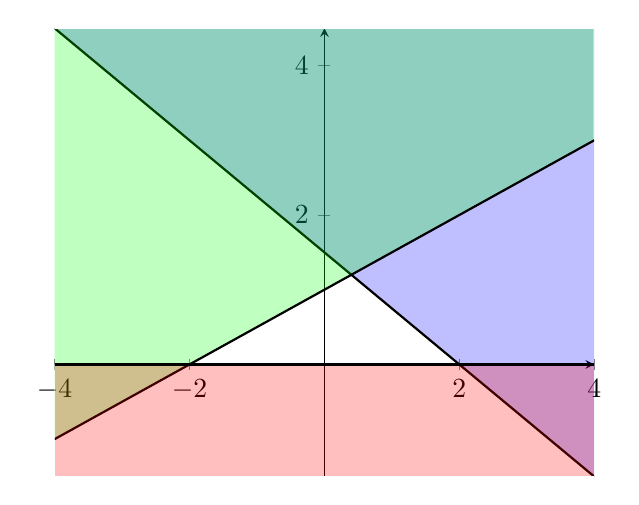
\begin{tikzpicture} 

    \begin{axis}[enlargelimits=0.1, axis lines=middle]
    % First one
    \addplot [color=white,fill=blue, 
              fill opacity=0.25]coordinates {
              (4,-1.5)
              (-4,4.5)
              (4,4.5)};
    \addplot[domain=-4:4,fill=gray!50, thick] {(6 - (3*x)) / 4};
    % Second one
    \addplot [color=white,fill=green, 
              fill opacity=0.25]coordinates {
              (-4,4.5)
              (4,4.5)
              (4,3)
              (-4,-1)};
    \addplot[domain=-4:4,fill=gray!50, thick] {(2 + x) / 2};
    % Third one
    \addplot [color=white,fill=red, 
              fill opacity=0.25]coordinates {
              (4,0)
              (-4,0)
              (-4,-1.5)
              (4,-1.5)};
    \addplot[domain=-4:4,fill=gray!50, thick] {0};
    \end{axis}
\end{tikzpicture}  
\end{document}